\subsection{Poiseuille's flow}
In order to test the periodic boundary conditions a one dimensional planar
Hagen-Poiseuille flow with an imposed pressure gradient was simulated and
compared to the analytical solution. The analytical solution is obtained
starting with the conservation of mass and momentum 
\begin{subequations}
    \begin{equation}
        \pdv{u}{x} + \pdv{v}{y} = 0
    \end{equation}
    \begin{equation}
        \pdv{u}{t} + \pdv{uu}{x} + \pdv{uv}{y} = 
                    - \pdv{p}{x} 
                    + \nu \left( \pdv{u}{x}{x} + \pdv{u}{y}{y} \right)  
        \label{eq:u-momentum}
    \end{equation}
    \begin{equation}
        \pdv{v}{t} + \pdv{uv}{x} + \pdv{vv}{y} = 
                    - \pdv{p}{y} 
                    + \nu \left( \pdv{v}{x}{x} + \pdv{v}{y}{y} \right)  
        \label{eq:v-momentum}
    \end{equation}
\end{subequations}

\begin{figure}[H]
    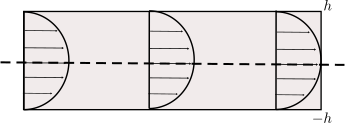
\includegraphics[width=0.5\textwidth]{../../../media/poiseuille-flow}
    \caption{Planar Hagen-Poiseuille flow}
\end{figure}

Where for steady one dimensional flow ($\mathbf{u} \equiv (u,v=0)$) 
the conservation of momentum reduces to    
\begin{equation}
    \nu \dv[2]{u}{y} = \dv{p}{x} = \text{const}
\end{equation}
Solving the above ODE and applying no slip boundary conditions at the
walls, $u(h)=u(-h)=0$, gives the exact analytical solution, namely 
\begin{subequations}
    \begin{equation}
        u(y) = u_{max} \left(1-\frac{y}{h^{2}}\right)
    \end{equation}
    \text{where}
    \begin{equation}
        u_{max} = -\dv{p}{x} \frac{h^2}{2\nu}
    \end{equation}
\end{subequations}

Figure~(\ref{fig:periodic-domain}) compares the cross sectional simulation
velocity profile to the exact Poiseuille flow solution.
\begin{figure}[H]
    \includegraphics[width=0.5\textwidth]{../data/data-64-dev/u-poiseuille.png}
    \caption{Cross sectional $u$ velocity}
    \label{fig:periodic-domain}
\end{figure}                                                            
